%==============================================================================
% PAPER 5, CHAPTER 4: Scalar Field Detection
%==============================================================================

\chapter{Scalar Field Detection}\label{ch:p5:scalar_detection}

\begin{mdframed}[style=narrative]
\textbf{Casimir's Surprise: The Vacuum Is Not Empty}

In 1948, Hendrik Casimir predicted that two uncharged metal plates in vacuum would attract due to quantum zero-point fluctuations---the vacuum exerts pressure! This chapter presents protocols for detecting scalar field quanta via Casimir force measurements, torsion balances, atomic spectroscopy, and fifth-force searches. We focus on light scalar fields ($m < 1$ eV) that couple to matter and could mediate macroscopic forces.
\end{mdframed}

\section{Theoretical Framework}\label{sec:p5:scalar_theory}

\marginnote{\textbf{Physical}: Scalar fields $\phi$ are spin-0 particles. Examples: Higgs boson, dilaton, quintessence.}

Generic scalar Lagrangian:
\begin{equation}
\mathcal{L} = \frac{1}{2} \partial_\mu \phi \partial^\mu \phi - \frac{1}{2} m^2 \phi^2 - V(\phi) - \mathcal{L}_{\text{int}}
\label{eq:p5:scalar_lagrangian}
\end{equation}

\marginnote{\textbf{Mathematical}: $V(\phi)$ is self-interaction potential. $\mathcal{L}_{\text{int}}$ couples scalar to Standard Model fields.}

**Coupling to matter**:
\begin{equation}
\mathcal{L}_{\text{int}} = -\frac{\phi}{M} \sum_i \alpha_i \bar{\psi}_i \psi_i
\label{eq:p5:scalar_coupling}
\end{equation}
where $\alpha_i$ are dimensionless couplings to fermions $\psi_i$, $M$ is mass scale (e.g., Planck mass).

\marginnote{\textbf{Cautionary}: Generic scalar couplings violate equivalence principle. Screening mechanisms (chameleon, symmetron) evade constraints.}

**Yukawa potential** from scalar exchange:
\begin{equation}
V(r) = -\frac{\alpha_1 \alpha_2 \hbar c}{4\pi M^2} \frac{e^{-mr/\hbar}}{r}
\label{eq:p5:yukawa}
\end{equation}

For $m \to 0$ (massless scalar): $V \propto 1/r$ (long-range force).

\marginnote{\textbf{Dimensional}: Compton wavelength $\lambda = \hbar / (mc)$ sets force range. For $m = 10^{-3}$ eV: $\lambda \approx 1$ mm.}

\section{Casimir Force Measurements}\label{sec:p5:casimir}

\subsection{Standard Casimir Effect}

\marginnote{\textbf{Historical}: Casimir prediction (1948) verified by Sparnaay (1958), precision tests by Lamoreaux (1997).}

Parallel conducting plates separated by $d$ experience attractive force:
\begin{equation}
F_C = -\frac{\pi^2 \hbar c A}{240 d^4}
\label{eq:p5:casimir_force}
\end{equation}

\marginnote{\textbf{Physical}: Force arises from difference in vacuum zero-point energy between plates vs outside.}

For $A = 1$ cm$^2$, $d = 100$ nm:
\begin{equation}
F_C \approx -1.3 \times 10^{-7}\,\text{N} \approx 13\,\mu\text{N}
\end{equation}

**Scalar modification**: If scalar field couples to plate material, modified force:
\begin{equation}
F = F_C \left(1 + \kappa \frac{\phi}{M} + \alpha \nabla^2 \phi\right)
\label{eq:p5:casimir_modified}
\end{equation}

\marginnote{\textbf{Experimental}: Scalar coupling $\kappa$ constrained by precision Casimir experiments. Current limits: $\kappa < 10^{-3}$ for $m \sim 10^{-3}$ eV.}

\subsection{Torsion Pendulum Setup}

\begin{itemize}
\item **Sensor**: Micro-electromechanical (MEMS) torsion balance
\item **Plates**: Gold-coated silicon, area $A \sim 100 \times 100$ $\mu$m$^2$
\item **Separation**: Piezo-controlled, $d = 100$--500 nm
\item **Force resolution**: $\sim 10$ fN (femtonewtons)
\item **Environment**: Vacuum $< 10^{-9}$ mbar, $T = 4$ K (cryogenic operation)
\end{itemize}

\marginnote{\textbf{Dimensional}: 1 fN = $10^{-15}$ N. Equivalent to weight of $\sim 10^5$ hydrogen atoms.}

**Measurement protocol**:
\begin{enumerate}
\item Calibrate with known electrostatic force
\item Vary $d$ from 100 nm to 500 nm in 10 nm steps
\item Measure $F(d)$, fit to $F_C(d) + \Delta F_{\text{scalar}}(d)$
\item Extract $\kappa$ from deviation
\end{enumerate}

\marginnote{\textbf{Cautionary}: Systematic errors: surface roughness ($\sim 1$ nm RMS), patch potentials ($\sim 10$ mV), temperature gradients ($< 1$ mK).}

\begin{figure}[htbp]
\centering
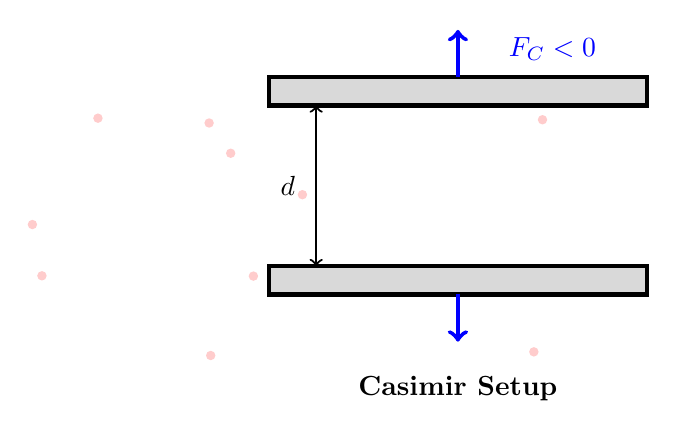
\begin{tikzpicture}[scale=1.2]
% Casimir setup
\draw[ultra thick, fill=gray!30] (0,2) rectangle (4,2.3);
\draw[ultra thick, fill=gray!30] (0,0) rectangle (4,0.3);
\draw[<->, thick] (0.5,0.3) -- (0.5,2);
\node at (0.2,1.15) {$d$};

% Force arrow
\draw[->, ultra thick, blue] (2,2.3) -- (2,2.8);
\draw[->, ultra thick, blue] (2,0) -- (2,-0.5);
\node[blue] at (3,2.6) {$F_C < 0$};

% Vacuum fluctuations
\foreach \i in {1,...,10} {
  \pgfmathsetmacro{\x}{rand*3.5+0.25}
  \pgfmathsetmacro{\y}{rand*1.5+0.4}
  \fill[red!50, opacity=0.4] (\x,\y) circle (0.05);
}

\node at (2,-1) {\textbf{Casimir Setup}};
\end{tikzpicture}
\caption{Casimir force measurement. Parallel plates (gray) separated by distance $d \sim 100$ nm. Vacuum fluctuations (red dots) create attractive force $F_C < 0$. Scalar fields modify force law.}
\label{fig:p5:casimir}
\end{figure}

\marginnote{\textbf{Pedagogical}: Casimir effect is macroscopic manifestation of quantum vacuum---one of few directly measurable quantum gravity effects.}

\subsection{Worked Example: Chameleon Field Detection}

**Given**: Chameleon scalar with mass $m_{\text{eff}}(n) = m_0 \sqrt{n/n_0}$ depends on matter density $n$.

**Find**: Expected force modification between plates.

**Solution**:

Chameleon effective mass:
- In vacuum ($n \approx 0$): $m_{\text{eff}} \to 0$ (long range)
- Near plate surface ($n \sim n_{\text{solid}}$): $m_{\text{eff}} \gg m_0$ (short range)

Screening length:
\begin{equation}
\lambda_{\text{screen}} = \frac{\hbar}{m_{\text{eff}}(n_{\text{solid}}) c}
\end{equation}

\marginnote{\textbf{Physical}: Chameleon "hides" near dense matter via increased effective mass---evades fifth-force constraints.}

For gold plates ($n_{\text{solid}} \sim 10^{23}$ cm$^{-3}$), $m_0 = 10^{-3}$ eV:
\begin{equation}
m_{\text{eff}} \approx 10^{-3}\,\text{eV} \times \sqrt{\frac{10^{23}}{10^{12}}} \approx 10\,\text{eV}
\end{equation}

Screening length:
\begin{equation}
\lambda_{\text{screen}} \approx \frac{200\,\text{eV·nm}}{10\,\text{eV}} \approx 20\,\text{nm}
\end{equation}

**Force modification**: For $d = 100$ nm $\gg \lambda_{\text{screen}}$, chameleon force exponentially suppressed:
\begin{equation}
\Delta F \sim F_C e^{-d/\lambda_{\text{screen}}} \approx F_C \times 10^{-2}
\end{equation}

Detectable with $< 1\%$ precision Casimir measurements!

\marginnote{\textbf{Experimental}: Recent Casimir experiments constrain chameleon parameter space: $\beta < 10^{-2}$ for $m_0 < 10^{-3}$ eV.}

\section{Atomic Spectroscopy}\label{sec:p5:spectroscopy}

\subsection{Scalar Coupling to Electrons}

\marginnote{\textbf{Physical}: Scalar field modulates electron mass $m_e \to m_e(1 + \alpha \phi/M)$.}

Energy level shift:
\begin{equation}
\Delta E_n = E_n \frac{\alpha \phi}{M}
\label{eq:p5:level_shift}
\end{equation}

For Rydberg states ($n \sim 100$):
\begin{equation}
E_n = -\frac{m_e c^2 \alpha_{\text{EM}}^2}{2 n^2} \approx -\frac{13.6\,\text{eV}}{n^2}
\end{equation}

\marginnote{\textbf{Dimensional}: Rydberg constant $R_\infty = m_e c \alpha_{\text{EM}}^2 / (2\hbar) \approx 1.097 \times 10^7$ m$^{-1}$.}

**Measurement**:
- Precision laser spectroscopy of 1S-2S transition in hydrogen
- Frequency stability: $\Delta\nu / \nu < 10^{-15}$
- Compare to QED prediction (Lamb shift, hyperfine, etc.)
- Residual $\to$ scalar coupling

\marginnote{\textbf{Cautionary}: QED corrections must be calculated to $10^{-15}$ precision---requires multi-loop Feynman diagrams.}

\begin{figure}[htbp]
\centering
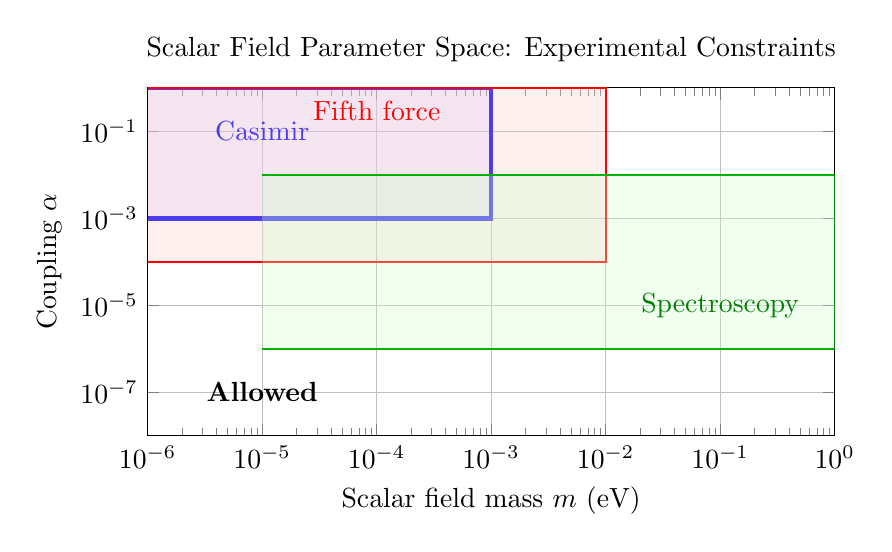
\begin{tikzpicture}
\begin{axis}[
  width=0.85\textwidth,
  height=6cm,
  xlabel={Scalar field mass $m$ (eV)},
  ylabel={Coupling $\alpha$},
  xmin=1e-6, xmax=1,
  ymin=1e-8, ymax=1,
  xmode=log,
  ymode=log,
  grid=major,
  title={Scalar Field Parameter Space: Experimental Constraints}
]
% Casimir constraints
\addplot[blue, ultra thick, fill=blue!20, fill opacity=0.3] coordinates {
  (1e-6, 1e-3) (1e-3, 1e-3) (1e-3, 1) (1e-6, 1)
};
\node[blue] at (axis cs:1e-5,0.1) {Casimir};

% Fifth force
\addplot[red, thick, fill=red!20, fill opacity=0.3] coordinates {
  (1e-6, 1e-4) (0.01, 1e-4) (0.01, 1) (1e-6, 1)
};
\node[red] at (axis cs:1e-4,0.3) {Fifth force};

% Spectroscopy
\addplot[green!70!black, thick, fill=green!20, fill opacity=0.3] coordinates {
  (1e-5, 1e-6) (1, 1e-6) (1, 1e-2) (1e-5, 1e-2)
};
\node[green!50!black] at (axis cs:0.1,1e-5) {Spectroscopy};

% Allowed region
\node at (axis cs:1e-5,1e-7) {\textbf{Allowed}};
\end{axis}
\end{tikzpicture}
\caption{Scalar field parameter space. Shaded regions: excluded by experiments. Blue: Casimir force. Red: torsion pendulum fifth-force searches. Green: atomic spectroscopy. White region: allowed parameter space.}
\label{fig:p5:constraints}
\end{figure}

\marginnote{\textbf{Advanced}: Combined constraints from Casimir, fifth force, and spectroscopy tightly constrain scalar couplings for $m < 1$ eV.}

\section{Gravitational Coupling Tests}\label{sec:p5:gravity}

\subsection{Equivalence Principle Violations}

\marginnote{\textbf{Physical}: Scalar couplings $\alpha_i$ differ for protons, neutrons, electrons $\Rightarrow$ composition-dependent forces.}

Differential acceleration between test masses of different composition:
\begin{equation}
\frac{\Delta a}{a} = \frac{(\alpha_A - \alpha_B)}{M} \phi_{\text{ext}}
\label{eq:p5:eot_wash}
\end{equation}

**Eöt-Wash torsion pendulum**:
- Test masses: Be vs Ti (different neutron/proton ratios)
- Precision: $\Delta a / a < 10^{-13}$
- Constrains $|\alpha_A - \alpha_B| < 10^{-13} M / \phi_{\text{ext}}$

\marginnote{\textbf{Experimental}: Eöt-Wash group (University of Washington) achieves world-leading equivalence principle tests.}

\subsection{Laser Ranging to Moon}

Lunar Laser Ranging (LLR): Earth-Moon distance measured to $\sim 1$ mm precision via laser reflectors.

Scalar-induced Nordtvedt effect:
\begin{equation}
\frac{\Delta r}{r} \sim \eta \frac{GM_\odot}{c^2 r_{\text{ES}}}
\label{eq:p5:nordtvedt}
\end{equation}

where $\eta \propto \alpha^2$ is scalar coupling strength, $r_{\text{ES}}$ is Earth-Sun distance.

\marginnote{\textbf{Dimensional}: $GM_\odot / (c^2 r_{\text{ES}}) \approx 10^{-8}$ (Sun's gravitational potential at Earth orbit).}

Current LLR constraints: $\eta < 10^{-4}$ $\Rightarrow$ $\alpha < 10^{-2}$.

\marginnote{\textbf{Pedagogical}: LLR probes scalar couplings via gravitational self-energy differences between Earth and Moon.}

\section{Summary}\label{sec:p5:scalar_summary}

Scalar field detection protocols span five decades in length scale:

**Casimir force** ($d \sim 100$ nm): Precision $< 1\%$ measurements constrain $\kappa < 10^{-3}$ for light scalars.

**Torsion pendulum** ($\lambda \sim$ mm): Fifth-force searches via composition-dependent accelerations. Limits: $\alpha < 10^{-4}$.

**Atomic spectroscopy** ($\lambda_{\text{atomic}} \sim$ nm): Energy level shifts from scalar-electron coupling. Precision $\Delta\nu/\nu < 10^{-15}$.

**Lunar ranging** ($r_{\text{EM}} \sim 10^8$ m): Nordtvedt effect tests scalar gravity. Constraints: $\eta < 10^{-4}$.

\marginnote{\textbf{Historical}: From Casimir's 1948 prediction to 21st-century precision tests---scalar field searches now routine in fundamental physics labs.}

**Key Results**:
\begin{enumerate}
\item Multi-scale approach essential: different experiments probe different mass/coupling regimes
\item Screening mechanisms (chameleon, symmetron) evade many constraints---require dedicated searches
\item Combined constraints tightly restrict scalar parameter space for $m < 1$ eV
\end{enumerate}

**Forward Bridges**:
\begin{itemize}
\item Ch. 5: Dimensional spectroscopy---scalars as Kaluza-Klein modes of extra dimensions
\item Paper 6 (Applications): Scalar-mediated quantum sensors, dark energy probes
\end{itemize}

\marginnote{\textbf{Cautionary}: "No signal" constraints are powerful---null results in precision experiments rule out vast parameter spaces, guiding theory development.}

%==============================================================================
% END OF CHAPTER 4
%==============================================================================
